
\de{ĐỀ THI GIỮA HỌC KỲ I NĂM HỌC 2022-2023}{THPT Trần Phú}
\begin{center}
	\textbf{PHẦN 1 - TRẮC NGHIỆM}
\end{center}
\Opensolutionfile{ans}[ans/ans]
\begin{ex}%[0D3Y2-1]%[Dự án đề kiểm tra GHKII NH22-23-VU Ngoc Hao]%[TRẦN PHÚ]
	Tam thức bậc hai nào sau đây luôn dương trên khoảng $(1;3)$?
	\choice
	{$x^2-4x+3$}
	{$x^2-3x+2$}
	{\True $x^2-2x+2$}
	{$x^2-2x-3$}
	\loigiai
	{Ta có $x^2-2x+2=(x-1)^2+1>0,\, \forall x\in \mathbb{R}$, do đó tam thức luôn dương với mọi $x\in (1;3)$.}
\end{ex}

\begin{ex}%[0D4B5-2]%[Dự án đề kiểm tra GHKII NH22-23-VU Ngoc Hao]%[TRẦN PHÚ]
	Tập xác định $\mathscr{D}$ của hàm số $y=\sqrt{5-4x-x^2}$ là
	\choice
	{\True $\mathscr{D}=[-5;1]$}
	{$\mathscr{D}=[-1;5)$}
	{$\mathscr{D}=(-5;1)$}
	{$\mathscr{D}=(-\infty;-5]\cup [1;+\infty)$}
	\loigiai
	{Hàm số xác định khi và chỉ khi $5-4x-x^2\geq 0$.\\
		Ta có $5-4x-x^2=0\Leftrightarrow \hoac{& x=1 \\ & x=-5}$ và bảng xét dấu của $5-4x-x^2$ như sau
		\begin{center}
			\begin{tikzpicture}
				\tkzTabInit[nocadre=false,lgt=3.5,espcl=2.5]
				{$x$ /0.6,$-x^2-4x+5$ /0.6}
				{$-\infty$,$-5$,$1$,$+\infty$}
				\tkzTabLine{,-,$0$,+,$0$,-,}
			\end{tikzpicture}
		\end{center}
		Do đó $-x^2-4x+5\geq 0 \Leftrightarrow -5\leq x\leq 1$.\\
		Vậy tập xác định của hàm số đã cho là $\mathscr{D}=[-5;1]$.}
\end{ex}

\begin{ex}%[1D2Y2-1]%[Dự án đề kiểm tra GHKII NH22-23-VU Ngoc Hao]%[TRẦN PHÚ]
	Một lớp có $50$ học sinh. Hỏi có bao nhiêu cách phân công $3$ bạn học sinh để trực nhật, biết rằng một bạn quét lớp, một bạn lau bảng và một bạn đổ rác.
	\choice
	{$128500$}
	{$19600$}
	{\True $117600$}
	{$376$}
	\loigiai
	{Mỗi cách chọn $3$ học sinh từ $50$ học sinh và phân công vào $3$ nhiệm vụ là một chỉnh hợp chập $3$ của $50$.\\
		Vậy có $\mathrm{A}_{50}^3 = 117600$ cách phân công.}
\end{ex}
\begin{ex}%[0D4Y5-1]%[Dự án đề kiểm tra GHKII NH22-23-VU Ngoc Hao]%[TRẦN PHÚ]
	Biểu thức nào sau đây là một tam thức bậc hai?
	\choice
	{\True $h(x)=-x^2+x+3$}
	{$g(x)=-2x+\dfrac{13}{2}$}
	{$f(x)=x^4-2x^2-3$}
	{$u(x)=\dfrac{1}{x}-3$}
	\loigiai
	{Biểu thức $h(x)=-x^2+x+3$ là một tam thức bậc hai.}
\end{ex}


\begin{ex}%[1D2Y1-2]%[Dự án đề kiểm tra GHKII NH22-23-VU Ngoc Hao]%[TRẦN PHÚ]
	Từ A đến B có $4$ con đường, từ B đến C có $3$ con đường. Hỏi có bao nhiêu cách chọn đường từ A đến C (phải qua B)?
	\choice
	{$64$}
	{\True $12$}
	{ $81$}
	{$7$}
	\loigiai
	{Có $4$ cách chọn một con đường từ A đến B. Mỗi cách chọn một con đường từ A đến B có $3$ cách chọn đường từ B đến C. Do đó có $4\cdot 3=12$ con đường đi từ A đến C (phải qua B).}
\end{ex}

\begin{ex}%[0D4B5-2]%[Dự án đề kiểm tra GHKII NH22-23-VU Ngoc Hao]%[TRẦN PHÚ]
	Với các giá trị nào của $m$ để bất phương trình $(2m-3)x^2-m^2x+2\geq 0$ nhận $x=-2$ là một nghiệm?
	\choice
	{$m\in [1;5]$}
	{$m\in (-\infty;1)$}
	{$m\in [-5;1]$}
	{\True $m\in (-\infty;-5]\cup [1;+\infty)$}
	\loigiai
	{Bất phương trình $(2m-3)x^2-m^2x+2\geq 0$ nhận $x=-2$ là một nghiệm khi
		$$(2m-3)\cdot (-2)^2+2m^2+2\geq 0 \Leftrightarrow m^2+4m-5\geq 0 \Leftrightarrow \hoac{& m\leq -5 \\ & m\geq 1.}$$}
\end{ex}

\begin{ex}%[0D4B5-6]%[Dự án đề kiểm tra GHKII NH22-23-VU Ngoc Hao]%[TRẦN PHÚ]
	Tập nghiệm của phương trình $\sqrt{x^2-x-2}=\sqrt{2x^2+x-1}$ là
	\choice
	{$S=\{-1;2\}$}
	{$S=\{3\}$}
	{\True $S=\{-1\}$}
	{$S=\{1\}$}
	\loigiai
	{Ta có
		\allowdisplaybreaks
		\begin{eqnarray*}
			&&\sqrt{x^2-x-2}=\sqrt{2x^2+x-1}\\
			& \Leftrightarrow & \heva{& x^2-x-2\geq 0 \\ & x^2-x-2=2x^2+x-1}\\
			& \Leftrightarrow & \heva{& x^2-x-2\geq 0 \\ & x^2+2x+1=0}\\
			& \Leftrightarrow & x=-1.
		\end{eqnarray*}
		Vậy tập nghiệm của phương trình là $S=\{-1\}$.}
\end{ex}


\begin{ex}%[0D4B5-6]%[Dự án đề kiểm tra GHKII NH22-23-VU Ngoc Hao]%[TRẦN PHÚ]
	Số nghiệm của phương trình $\sqrt{-2x+8}-x+6=x$ là
	\choice
	{$0$}
	{\True $1$}
	{ $2$}
	{$3$}
	\loigiai
	{Điều kiện $-2x+8\geq 0 \Leftrightarrow x\leq 4$. Ta có
		\allowdisplaybreaks
		\begin{eqnarray*}
			&&\sqrt{-2x+8}-x+6=x \\
			&\Leftrightarrow & \sqrt{-2x+8}=2x-6 \\
			&\Leftrightarrow & \heva{& 2x-6\geq 0 \\ & -2x+8=(2x-6)^2} \\
			&\Leftrightarrow & \heva{& x\geq 3 \\ & 4x^2-22x+28=0} \\
			&\Leftrightarrow & x=\dfrac{7}{2} \text{ (thỏa mãn)}.
		\end{eqnarray*}
		Vậy phương trình đã cho có nghiệm duy nhất $x=\dfrac{7}{2}$.}
\end{ex}

\begin{ex}%[0D4B5-2]%[Dự án đề kiểm tra GHKII NH22-23-VU Ngoc Hao]%[TRẦN PHÚ]
	Với các giá trị nào của $m$ thì bất phương trình $-3x^2+2mx+m^2\geq 0$ đúng với mọi $x\in \mathbb{R}$?
	\choice
	{$m\in\mathbb{R}\setminus \{0\}$}
	{\True $m\in \varnothing$}
	{$m\in \mathbb{R}$}
	{$m=0$}	
	\loigiai
	{Bất phương trình $-3x^2+2mx+m^2\geq 0$ đúng với mọi $x\in \mathbb{R}$ khi và chỉ khi
		$$\heva{& -3>0 \\ & \Delta'=m^2+3m^2\leq 0} \Leftrightarrow \text{ không tồn tại } m.$$}
\end{ex}

\begin{ex}%[1D2B1-2]%[Dự án đề kiểm tra GHKII NH22-23-VU Ngoc Hao]%[TRẦN PHÚ]
	Từ các chữ số $\{0;1;2;3;4;5;6\}$ có thể lập được bao nhiêu số tự nhiên có $3$ chữ số đôi một khác nhau?
	\choice
	{\True $180$}
	{$120$}
	{$60$}
	{$210$}
	\loigiai
	{Gọi số tự nhiên cần lập có dạng $\overline{abc}$ ($a\neq 0$). Khi đó có $6$ cách chọn chữ số $a$, $6$ cách chọn chữ số $b$ và $5$ cách chọn chữ số $c$.\\
		Vậy có thể lập được $6\cdot 6\cdot 5 = 180$ số thoả mãn yêu cầu.}
\end{ex}
\begin{ex}%[1D2B1-2]%[Dự án đề kiểm tra GHKII NH22-23-VU Ngoc Hao]%[TRẦN PHÚ]
	Để chuẩn bị cho tiết mục biểu diễn, anh hề phải chọn trang phục biểu diễn gồm mũ, tóc giả, mũi hề và quần áo. Đoàn xiếc có $10$ chiếc mũ, $6$ bộ tóc giả, $5$ cái mũi hề và $8$ bộ quần áo. Hỏi anh hề có bao nhiêu cách chọn trang phục biểu diễn?
	\choice
	{$240$}
	{$300$}
	{\True $2400$}
	{$29$}
	\loigiai
	{Số cách chọn trang phục biểu diễn của anh hề là số cách chọn $1$ chiếc mũ, $1$ bộ tóc giả, $1$ chiếc mũi hề và $1$ bộ quần áo.\\
		Vậy có $10\cdot 6\cdot 5\cdot 8 = 2400$ cách chọn trang phục biểu diễn của anh hề.}
\end{ex}
\begin{ex}%[0D2Y3-1]%[Dự án đề kiểm tra GHKII NH22-23-VU Ngoc Hao]%[TRẦN PHÚ]
	\immini
	{Cho hàm số $y=f(x)$ có đồ thị như hình vẽ bên. Hãy so sánh $f(2023)$ với số $0$.
		\choice[2]
		{\True $f(2023)<0$}
		{$f(2023)>0$}
		{$f(2023)\leq 0$}
		{$f(2023)\geq 0$}
	}
	{\begin{tikzpicture}[scale=1, font=\footnotesize, line join=round, line cap=round, >=stealth]
			\draw[->](-2,0) -- (0,0)node[below left]{$O$} -- (3,0)node[below]{$x$};
			\draw[->](0,-1)--(0,3)node[left]{$y$};
			\begin{scope}
				\clip (-2,-1) rectangle (3,3);
				\draw[smooth,samples=150] plot[domain=-2:3](\x,{-(\x+1)*(\x-2)});
			\end{scope}
			\foreach \i in {(-1,0),(2,0),(0,2)} \fill \i circle(1pt);
			\draw[dashed](-1,0)node[below left]{$-1$}
			(0,2)node[left]{$2$}
			(2,0)node[below right]{$2$};
	\end{tikzpicture}}
	\loigiai
	{Hàm số nghịch biến trên $[2;+\infty)$ nên $f(2023)<f(2)=0$.}
\end{ex}

\begin{ex}%[0D4B5-2]%[Dự án đề kiểm tra GHKII NH22-23-VU Ngoc Hao]%[TRẦN PHÚ]
	Số giá trị nguyên của $x$ thỏa mãn bất phương trình $2x^2-7x-9<0$ là
	\choice
	{$3$}
	{$4$}
	{\True $5$}
	{$6$}
	\loigiai
	{Ta có $2x^2-7x-9<0 \Leftrightarrow -1<x<\dfrac{9}{2}$.\\
		Do $x$ là nghiệm nguyên của bất phương trình nên $x\in \{0;1;2;3;4\}$.\\
		Vậy có $5$ giá trị của $x$ thỏa mãn.}
\end{ex}

\begin{ex}%[0D4B5-2]%[Dự án đề kiểm tra GHKII NH22-23-VU Ngoc Hao]%[TRẦN PHÚ]
	Phương trình $mx^2-2mx+4=0$ vô nghiệm khi và chỉ khi
	\choice
	{\True $0\leq m<4$}
	{$\hoac{& m\leq 0 \\ & m\geq 4}$}
	{$0<m<4$}
	{$\hoac{& m<0 \\ & m>4}$}
	\loigiai
	{Nếu $m=0$, phương trình $4=0$ vô nghiệm.\\
		Nếu $m\neq 0$ thì phương trình vô nghiệm khi và chỉ khi $\Delta'=m^2-4m<0$. Ta có bảng xét dấu $\Delta'$ như sau
		\begin{center}
			
\begin{tikzpicture}
				\tkzTabInit[nocadre=false,lgt=2,espcl=2]
				{$m$ /0.6,$m^2-4m$ /0.6}
				{$-\infty$,$0$,$4$,$+\infty$}
				\tkzTabLine{,+,0,-,0,+,}
			\end{tikzpicture}
		\end{center}
		Do đó $\Delta'<0  \Leftrightarrow 0<m<4$.\\
		Vậy phương trình đã cho vô nghiệm khi và chỉ khi $0\leq m<4$.}
\end{ex}

\begin{ex}%[0H3Y1-1]%[Dự án đề kiểm tra GHKII NH22-23-VU Ngoc Hao]%[TRẦN PHÚ]
	Cho đường thẳng $d\colon 2x+3y-4=0$, véc-tơ pháp tuyến của đường thẳng $d$ là
	\choice
	{$\overrightarrow{n}_1=(3;2)$}
	{\True $\overrightarrow{n}_2=(2;3)$}
	{$\overrightarrow{n}_3=(3;-2)$}
	{$\overrightarrow{n}_4=(-2;3)$}
	\loigiai
	{Véc-tơ pháp tuyến của đường thẳng $d$ là $\overrightarrow{n}_2=(2;3)$.}
\end{ex}

\begin{ex}%[0H3Y1-6]%[Dự án đề kiểm tra GHKII NH22-23-VU Ngoc Hao]%[TRẦN PHÚ]
	Cho đường thẳng $d\colon \heva{& x=2-3t \\ & y=-1+2t}$ và điểm $A(-1;1)$. Điểm $A\in d$ ứng với giá trị nào của $t$?
	\choice
	{\True $t=1$}
	{$t=2$}
	{$t=-1$}
	{$t=0$}
	\loigiai
	{Ta có $A\in d \Leftrightarrow \heva{& -1=2-3t \\ & 1=-1+2t} \Leftrightarrow t=1$.}
\end{ex}


\begin{ex}%[0H2Y2-2]%[Dự án đề kiểm tra GHKII NH22-23-VU Ngoc Hao]%[TRẦN PHÚ]
	Trong mặt phẳng tọa độ $Oxy$, cho hai điểm $A(3;1)$, $B(2;-6)$. Độ dài đoạn thẳng $AB$ bằng
	\choice
	{$AB=50$}
	{$AB=5$}
	{$AB=2\sqrt{5}$}
	{\True $AB=5\sqrt{2}$}
	\loigiai
	{Ta có $AB=\sqrt{(2-3)^2+(-6-1)^2} = \sqrt{50} = 5\sqrt{2}$.}
\end{ex}

\begin{ex}%[0H3B1-4]%[Dự án đề kiểm tra GHKII NH22-23-VU Ngoc Hao]%[TRẦN PHÚ]
	Trong mặt phẳng tọa độ $Oxy$, cho đường thẳng $d\colon \heva{& x=1+t \\ & y=-3+2t}$ và đường thẳng $\Delta\colon \heva{& x=1+2t' \\ & y=1+t'}$. Tính cô-sin của góc giữa hai đường thẳng $d$ và $\Delta$.
	\choice
	{$\dfrac{1}{5}$}
	{\True $\dfrac{4}{5}$}
	{$\dfrac{4}{\sqrt{5}}$}
	{$\dfrac{1}{\sqrt{5}}$}
		\loigiai
	{Đường thẳng $d$ có véc-tơ chỉ phương $\overrightarrow{u}=(1;2)$, đường thẳng $\Delta$ có véc-tơ chỉ phương $\overrightarrow{v}=(2;1)$ nên
		$$\cos\left(d,\Delta\right) = \left| \cos\left(\overrightarrow{u}, \overrightarrow{v}\right) \right| = \dfrac{\left| \overrightarrow{u} \cdot \overrightarrow{v}\right|}{\left| \overrightarrow{u} \right| \cdot \left| \overrightarrow{v}\right|} = \dfrac{\left| 2+2\right|}{\sqrt{2^2+1^2} \cdot \sqrt{1^2+2^2}} = \dfrac{4}{5}.$$}
\end{ex}

\begin{ex}%[0H3B1-2]%[Dự án đề kiểm tra GHKII NH22-23-VU Ngoc Hao]%[TRẦN PHÚ] 
	Trong mặt phẳng tọa độ $Oxy$, phương trình tham số của đường thẳng đi qua hai điểm $M(3;5)$ và $N(6;2)$ là
	\choice
	{$x+y-8=0$}
	{$\heva{& x=3+t \\ & y=5+t}$}
	{\True $\heva{& x=3+t \\ & y=5-t}$}
	{$\heva{& x=6-t \\ & y=2-t}$}
	\loigiai
	{Đường thẳng $MN$ nhận véc-tơ $\overrightarrow{MN}=(3;-3)$ làm véc-tơ chỉ phương nên cũng nhận véc-tơ $\overrightarrow{u}=(1;-1)$ làm véc-tơ chỉ phương.\\
		Vậy phương trình tham số của đường thẳng $MN$ là $\heva{& x=3+t \\ & y=5-t.}$}
\end{ex}


\begin{ex}%[0H3Y1-6]%[Dự án đề kiểm tra GHKII NH22-23-VU Ngoc Hao]%[TRẦN PHÚ]
	Tọa độ hình chiếu vuông góc của điểm $B(-2;5)$ trên trục hoành $Ox$ là
	\choice
	{$(2;5)$}
	{\True $(-2;0)$}
	{$(0;5)$}
	{$(5;0)$}
	\loigiai
	{Tọa độ hình chiếu của điểm $B(-2;5)$ trên trục $Ox$ là $(-2;0)$.}
\end{ex}


\Closesolutionfile{ans}
%\begin{center}
%	\textbf{ĐÁP ÁN}
%	\inputansbox{10}{ans/ans}	
%\end{center}
\begin{center}
	\textbf{PHẦN 2 - TỰ LUẬN}
\end{center}
%%%% Bài 1
\begin{bt}%[0T7B2-3]%[Dự án đề kiểm tra GKII NH22-23 - Thành Đức Trung]%[THPT Trần Phú - Hồ Chí Minh]
Giải bất phương trình sau $\left(x^2-7x+12\right)\left(9-x^2\right)\leqslant0$.
\loigiai
{\\
Ta có $\left(x^2-7x+12\right)\left(9-x^2\right)\leqslant0 \Leftrightarrow (x-3)(x-4)(x-3)(x+3)\geqslant0 \Leftrightarrow \left(x-3\right)^2(x-4)(x+3)\geqslant0$. \hfill $(1)$ \\
Đặt $f(x)=\left(x-3\right)^2(x-4)(x+3)$. \\
Xét $f(x)=0 \Leftrightarrow \left(x-3\right)^2(x-4)(x+3)=0 \Leftrightarrow \hoac{ & x=3 \\ & x=4 \\ & x=-3.}$ \\
Bảng xét dấu của $f(x)$
\begin{center}

\begin{tikzpicture}[scale=1, >=stealth]
\tkzTabInit[nocadre=false, lgt=1.2, espcl=2.5, deltacl=0.6]{$x$/0.6, $f(x)$/0.6}{$-\infty$, $-3$, $3$, $4$, $+\infty$}
\tkzTabLine{,+,0,-,0,-,0,+,}
\end{tikzpicture}
\end{center}
Từ bảng xét dấu của $f(x)$ ta có $(1) \Leftrightarrow \hoac{ & x\leqslant-3 \\ & x=3 \\ & x\geqslant4.}$ \\
Vậy bất phương trình đã cho có tập nghiệm là $S=(-\infty;-3]\cup\{3\}\cup[4;+\infty)$.
}
\end{bt}

%%%% Bài 2
\begin{bt}%[0T7B1-2]%[Dự án đề kiểm tra GKII NH22-23 - Thành Đức Trung]%[THPT Trần Phú - Hồ Chí Minh]
Tìm $m$ để bất phương trình $-x^2+2(m-1)x+6\left(m^2-3m+2\right)<0$ có tập nghiệm là $\mathbb{R}$.
\loigiai
{\\
Yêu cầu bài toán tương đương với
$$\begin{aligned}
& \ -x^2+2(m-1)x+6\left(m^2-3m+2\right)<0, \forall x\in\mathbb{R} \\
\Leftrightarrow & \ \heva{ & a=-1<0 \ (\text{luôn đúng}) \\ & \Delta'=\left(m-1\right)^2+6\left(m^2-3m+2\right)<0} \\
\Leftrightarrow & \ 7m^2-20m+13<0 \\
\Leftrightarrow & \ 1<m<\dfrac{13}{7}.
\end{aligned}$$
Vậy $1<m<\dfrac{13}{7}$.
}
\end{bt}

%%%% Bài 3
\begin{bt}%[0T7K3-4]%[Dự án đề kiểm tra GKII NH22-23 - Thành Đức Trung]%[THPT Trần Phú - Hồ Chí Minh]
\immini
{
Một người chạy bộ từ vị trí $A$ đến vị trí $C$ trên đoạn đường $BD$, sau đó đạp xe từ vị trí $C$ đến vị trí $B$. Biết rằng vận tốc chạy bộ là $6$km/h, vận tốc đạp xe là $8$km/h, khoảng cách từ vị trí $A$ đến đoạn đường $BD$ bằng $3$km, khoảng cách giữa hai vị trí $B$ và $D$ bằng $8$km. Tính khoảng cách lớn nhất giữa hai vị trí $B$, $C$ biết rằng tổng thời gian người đó chạy bộ và đạp xe là $1$ giờ $20$ phút.
}
{
\begin{tikzpicture}[scale=1, font=\footnotesize, line join=round, line cap=round, >=stealth]
\path
(0,0)coordinate(D)
(8,0)coordinate(B)
(20/7,0)coordinate(C)
(0,3)coordinate(A)
($(A)!0.5!(D)$)node[left]{$3$km}
($(B)!0.5!(D)-(0,0.5)$)node[below]{$8$km}
;
\draw(A)--(D)--(B)--(A)--(C);
\draw[<->, dashed]($(D)-(0,0.5)$)--($(B)-(0,0.5)$);
\foreach \p/\q in {A/90, D/-90, B/-90, C/-90} \fill[black] (\p) circle (2pt) ($(\p)+(\q:2.5mm)$) node{$\p$};
\end{tikzpicture}
}
\loigiai
{\\
Đặt $CD=x$ ($0\leqslant x\leqslant8$; đơn vị km), suy ra $BC=8-x$ (km). \\
Ta có $AC=\sqrt{AD^2+CD^2}=\sqrt{x^2+9}$ (km). \\
Thời gian chạy bộ là $\dfrac{\sqrt{x^2+9}}{6}$ (giờ). \\
Ta có $1$ giờ $20$ phút bằng $\dfrac{4}{3}$ giờ. \\
Suy ra thời gian đạp xe là $\dfrac{4}{3}-\dfrac{\sqrt{x^2+9}}{6}=\dfrac{8-\sqrt{x^2+9}}{6}$ (giờ). \\
Do đó $BC=8\cdot\dfrac{8-\sqrt{x^2+9}}{6}=\dfrac{32-4\sqrt{x^2+9}}{3}$ (km). \\
Ta có phương trình $8-x=\dfrac{32-4\sqrt{x^2+9}}{3} \Leftrightarrow 4\sqrt{x^2+9}=3x+8$. \hfill $(1)$ \\
Bình phương hai vế phương trình $(1)$ ta có $16\left(x^2+9\right)=\left(3x+8\right)^2 \Leftrightarrow 7x^2-48x+80=0 \Leftrightarrow \hoac{ & x=4 \\ & x=\dfrac{20}{7}.}$ \\
Thay thử lại vào phương trình $(1)$ ta thấy hai nghiệm $x=4$, $x=\dfrac{20}{7}$ thỏa mãn. \\
Với $x=4$ ta có $BC=4$ (km). \\
Với $x=\dfrac{20}{7}$ ta có $BC=\dfrac{36}{7}$ (km). \\
Vậy khoảng cách lớn nhất giữa hai vị trí $B$, $C$ là $\dfrac{36}{7}$km. \\
}
\end{bt}

%%%% Bài 4
\begin{bt}%[0T9B2-5]%[0T9B2-6]%[Dự án đề kiểm tra GKII NH22-23 - Thành Đức Trung]%[THPT Trần Phú - Hồ Chí Minh]
Trong mặt phẳng $Oxy$, cho điểm $A(2;1)$ và đường thẳng $d\colon x-2y+2=0$.
\begin{enumerate}
\item Tính khoảng cách từ điểm $A$ đến đường thẳng $d$.
\item Tìm tọa độ hình chiếu $H$ của điểm $A$ lên đường thẳng $d$.
\end{enumerate}
\loigiai
{
\begin{enumerate}
\item Khoảng cách từ điểm $A$ đến đường thẳng $d$ là $\mathrm{d}(A,d)=\dfrac{|2-2\cdot1+2|}{\sqrt{1^2+\left(-2\right)^2}}=\dfrac{2\sqrt{5}}{5}$.
\item Ta có $AH\perp d$ nên $AH$ có phương trình dạng $2x+y+C=0$. \\
Vì $AH$ đi qua $A$ nên $2\cdot2+1+C=0 \Leftrightarrow C=-5$, suy ra phương trình $AH\colon 2x+y-5=0$. \\
Vì $H$ là giao điểm của $AH$ và $d$ nên tọa độ của $H$ là nghiệm của hệ phương trình
$$\heva{ & 2x+y-5=0 \\ & x-2y+2=0} \Leftrightarrow \heva{ & x=\dfrac{8}{5} \\ & y=\dfrac{9}{5}.}$$
Vậy $H\left(\dfrac{8}{5};\dfrac{9}{5}\right)$.
\end{enumerate}
}
\end{bt}